In the following sections we will introduce some mathematical notation and
definitions and present important theorems and algorithms from the field of
computational group theory. In each of these sections we will first introduce
some mathematical object via a series of definitions and then discuss
algorithms and data structures with which we can construct and represent
instances of this object in a computer program. Hereby we lay the foundation we
need to formalize the TMOR problem in Section~\ref{sec:tmor_definition} and to
understand the algorithms presented in
Section~\ref{sec:tmor_algorithmic_approaches} that address it.

Sections~\ref{sec:theo_permutations} and~\ref{sec:theo_permutation_groups} will
introduce permutations and permutation groups with which we can represent
symmetries inherent in MPSoC architectures.
Sections~\ref{sec:theo_partial_permutations}
and~\ref{sec:theo_partial_permutation_inverse_monoids} will introduce partial
permutations and partial permutation inverse monoids with which we can
represent partial symmetries as well, making them potentially more powerful.

For general literature on group theory including permutations and permutation
groups, refer to \cite{Rotman}. For an extensive treatment of inverse monoids
refer to \cite{Lawson} and for a comprehensive overview of computational group
theory refer to \cite{Holt}, \cite{Butler} and \cite{Seress}.

\section{Permutations}
\label{sec:theo_permutations}

\subsection{Motivation}
\label{sec:perm_motivation}

Permutations are a useful mathematical tool when it comes to describing
symmetries of systems. To illustrate this point, let us consider
\textit{isomorphisms} and \textit{automorphisms} of undirected\footnote{ While
we only consider undirected graphs here for simplicity, the following concepts
can easily be extended to directed graphs as well.} graphs and how we can
describe them mathematically.

\begin{defn}[label=exmp:undirected_graph]{Undirected Graph}
  An undirected graph is a tuple $G = (V,E)$ where $V = \{1,2,\dots,n \mid n
  \in \mathbb{N}\}$ is a set of vertex indices and $E \subseteq \{\{x, y\} \mid
  i, j \in V\}$ with $\{i, j\} \in E \Leftrightarrow$ a graph edge exists between
  the $i$th and $j$th vertex.
\end{defn}
%

\begin{exmp}[label=exmp:undirected_graph]{Undirected Graph}
  Consider the undirected graph $G = (V, E)$, with $V = \{1,2,3,4\}$ and $E =
  \{\{1,2\},\{2,3\},\{3,4\},\{4,1\}\}$ visualized in
  Figure~\ref{fig:undirected_graph}.
  %
  \begin{figure}[H]
    \centering
    \begin{tikzpicture}
      % vertices
      \Vertex[x=0,y=0,L=$1$]{1}
      \Vertex[x=1.5,y=0,L=$2$]{2}
      \Vertex[x=1.5,y=-1.5,L=$3$]{3}
      \Vertex[x=0,y=-1.5,L=$4$]{4}
      % edges
      \Edge(1)(2)
      \Edge(2)(3)
      \Edge(3)(4)
      \Edge(4)(1)
    \end{tikzpicture}
    \caption{An undirected graph with four vertices and edges.}
    \label{fig:undirected_graph}
  \end{figure}
\end{exmp}

\begin{defn}{Graph Isomorphism}
  Given two undirected graphs $G = (V_G, E_G)$ and $H = (V_H, E_H)$, an
  isomorphism is a bijective function $\operatorname{isom}: V_G \rightarrow V_H$
  with $\{i,j\} \in E_G \Leftrightarrow
  \{\operatorname{isom}(i),\operatorname{isom}(j)\} \in E_H$. If such a function
  exists we also say that $G$ and $H$ are isomorphic.
\end{defn}

\begin{exmp}{Graph Isomorphism}
  Consider the two undirected graphs $G = (V_G, E_G)$ and $H = (V_H, E_H)$
  visualized in Figure~\ref{fig:undirected_graph_isomorphism}.
  %
  \begin{figure}[H]
    \centering
    \begin{subfigure}{.3\textwidth}
      \centering
      \begin{tikzpicture}
        % vertices
        \Vertex[x=0,y=0,L=$1$]{1}
        \Vertex[x=1.5,y=0,L=$2$]{2}
        \Vertex[x=1.5,y=-1.5,L=$3$]{3}
        \Vertex[x=0,y=-1.5,L=$4$]{4}
        % edges
        \Edge(1)(2)
        \Edge(1)(3)
        \Edge(2)(3)
        \Edge(3)(4)
      \end{tikzpicture}
      \caption{$G$}
    \end{subfigure}
    %
    \begin{subfigure}{.3\textwidth}
      \centering
      \begin{tikzpicture}
        % vertices
        \Vertex[x=0,y=0,L=$1$]{1}
        \Vertex[x=1.5,y=0,L=$2$]{2}
        \Vertex[x=1.5,y=-1.5,L=$3$]{3}
        \Vertex[x=0,y=-1.5,L=$4$]{4}
        % edges
        \Edge(1)(4)
        \Edge(2)(3)
        \Edge(2)(4)
        \Edge(3)(4)
      \end{tikzpicture}
      \caption{$H$}
    \end{subfigure}
    \caption{Two isomorphic graphs.}
    \label{fig:undirected_graph_isomorphism}
  \end{figure}
  %
  \noindent
  The function $\operatorname{isom}: V_G \rightarrow V_H$ with:
  %
  \begin{equation*}
    \operatorname{isom}(1) = 2,\ \operatorname{isom}(2) = 3,\
    \operatorname{isom}(3) = 4,\ \operatorname{isom}(4) = 1
  \end{equation*}
  %
  is an isomorphism from $G$ to $H$. We can easily see that this is true by
  verifying that $\{\{\operatorname{isom}(i), \operatorname{isom}(j)\} \mid \{i,
  j\} \in E_G\} = E_H$:
  %
  \begin{align*}
    E_G = \{\{1,2\},\{1,3\}&,\{2,3\},\{3,4\}\} \\
                           &\symbolwithin{\Downarrow}{,} \\
    E_H = \{\{2,3\},\{2,4\}&,\{3,4\},\{4,1\}\}
  \end{align*}
  %
  Note that isomorphisms are \textit{structure preserving}, i.e. $G$ and $H$
  are the same graph aside from the differently numbered vertices.
\end{exmp}

\begin{defn}[label=defn:graph_automorphisms]{Graph Automorphism}
  Given an undirected graph ${G = (V, E)}$, an automorphism of $G$
  ${\operatorname{autom}: V \rightarrow V}$ is an isomorphism from $G$ to itself.
\end{defn}

\begin{exmp}[label=exmp:graph_automorphisms]{Graph Automorphism}
  Consider again the undirected graph $G$ from
  Example~\ref{exmp:undirected_graph} and the function ${\operatorname{autom}: V
  \rightarrow V}$ with:
  %
  \begin{equation*}
    \operatorname{autom}(1) = 2,\ \operatorname{autom}(2) = 3,\
    \operatorname{autom}(3) = 4,\ \operatorname{autom}(4) = 1
  \end{equation*}
  %
  Renumbering the vertices of $G$ according to $\operatorname{autom}$ results
  in the graph $G'$ visualized in
  Figure~\ref{fig:undirected_graph_automorphism_b}.
  %
  \begin{figure}[H]
    \centering
    \begin{subfigure}{.3\textwidth}
      \centering
      \begin{tikzpicture}[baseline=(current bounding box.center)]
        % vertices
        \Vertex[x=0,y=0,L=$1$]{1}
        \Vertex[x=1.5,y=0,L=$2$]{2}
        \Vertex[x=1.5,y=-1.5,L=$3$]{3}
        \Vertex[x=0,y=-1.5,L=$4$]{4}
        % edges
        \Edge(1)(2)
        \Edge(2)(3)
        \Edge(3)(4)
        \Edge(4)(1)
        % arrow
        \Vertex[empty,x=1,y=0.75]{x}
        \Vertex[empty,x=2.25,y=-0.5]{y}
        \tikzstyle{EdgeStyle}=[post, bend angle=45, bend left, style=thick]
        \Edge[color=red](x)(y)
        % dummy
        \Vertex[empty,x=-0.75,y=-0.5]{z}
      \end{tikzpicture}
      \caption{$G$}
      \label{fig:undirected_graph_automorphism_a}
    \end{subfigure}
    %
    \begin{subfigure}{.3\textwidth}
      \centering
      \begin{tikzpicture}[baseline=(current bounding box.center)]
        % vertices
        \Vertex[x=0,y=0,L=$4$]{1}
        \Vertex[x=1.5,y=0,L=$1$]{2}
        \Vertex[x=1.5,y=-1.5,L=$2$]{3}
        \Vertex[x=0,y=-1.5,L=$3$]{4}
        % edges
        \Edge(1)(2)
        \Edge(2)(3)
        \Edge(3)(4)
        \Edge(4)(1)
        % dummy
        \Vertex[empty,x=1,y=0.75]{x}
        \Vertex[empty,x=2.25,y=-0.5]{y}
        \Vertex[empty,x=-0.75,y=-0.5]{z}
      \end{tikzpicture}
      \caption{$G'$}
      \label{fig:undirected_graph_automorphism_b}
    \end{subfigure}
    \caption{A graph automorphism.}
  \end{figure}
  %
  \noindent
  Notice that this graph and $G$ are not only isomorphic but
  \textit{identical}, making $\operatorname{autom}$ an automorphism of $G$.
  Geometrically, if we interpret the vertices of $G$ as the edges of a square, we
  can view $\operatorname{autom}$ as a 90\degree\ right rotation of that
  square about its center (as indicated by the red arrow in
  Figure~\ref{fig:undirected_graph_automorphism_a}).
\end{exmp}
%
Graph automorphisms can thus express symmetries, e.g. rotational symmetry in
Example~\ref{exmp:graph_automorphisms}, inherent in a graph. As per
Definition~\ref{defn:graph_automorphisms}, every automorphism is a bijective
function from a set to itself. Such functions are exactly the permutations that
this section is concerned with.

\subsection{Definition}
\label{subsec:perm_definition}

\begin{defn}{Permutation}
  A permutation is a bijection from a set $\Omega$ to itself.
\end{defn}
%
We say that a permutation $g$ stabilizes some $x \in \Omega$ if $g(x) = x$ and
denote the \textit{identity permutation} that stabilizes all $x \in \Omega$
by $1$.

We usually denote permutations with the letters $g$ and $h$ and notate them in
either \textit{two-line notation} or \textit{cycle notation}. The former
displays $x$ and $g(x)$ on top of each other for each $x \in \Omega$ in a $2
\times |\Omega|$ matrix. The latter denotes a permutation as a sequence of
disjoint cycles where each element in a cycle is mapped to the next one by $g$
(in a cyclic fashion) and cycles of length one are omitted. We denote the
identity permutation as $()$ in cycle notation.

In the context of this thesis we are mostly concerned with the case $\Omega
\subseteq \mathbb{N}_+$, or more specifically $\Omega = \Omega_n = \{1, 2,
\dots, n\}$ where we refer to $n$ as the \textit{degree} of permutations of
$\Omega_n$. Unless otherwise noted, it is assumed that $\Omega$ has this form
and we also write $\operatorname{deg}(g)$ instead of $n$.

\begin{exmp}[label=exmp:permutation]{Permutation}
  Let $g: \Omega_5 \rightarrow \Omega_5$ such that:
  %
  \begin{equation*}
    g(1) = 2,\ g(2) = 1,\ g(3) = 3,\ g(4) = 5,\ g(5) = 4
  \end{equation*}
  %
  Then we can more compactly write $g$ as:
  %
  \begin{equation*}
    g = \begin{pmatrix} 1 & 2 & 3 & 4 & 5 \\ 2 & 1 & 3 & 5 & 4 \end{pmatrix}
  \end{equation*}
  %
  or:
  %
  \begin{equation*}
    g = (1\ 2)(4\ 5)
  \end{equation*}
\end{exmp}
%
Two more important concepts are the \textit{composition} of two permutations
and the \textit{inverse} of a permutation:

\begin{defn}{Permutation Composition}
  The composition of two permutations $g, h: \Omega \rightarrow \Omega$ is
  another permutation $gh: \Omega \rightarrow \Omega$ such that $\forall x \in
  \Omega: gh(x) = g(h(x))$. Note that this operation is associative but not
  commutative.
\end{defn}

\begin{defn}[label=defn:permutation_inverse]{Permutation Inverse}
  The inverse of a permutation $g: \Omega \rightarrow \Omega$ is another
  permutation $g^{-1}: \Omega \rightarrow \Omega$ such that $gg^{-1} = g^{-1}g =
  1$.
\end{defn}

\begin{exmp}{Permutation Inverse}
  Let $g$ be as in Example~\ref{exmp:permutation} and $h = (1\ 2\ 3\ 4)$ Then
  we have:
  %
  \begin{equation*}
    \begin{split}
      gh &= \begin{pmatrix} 1 & 2 & 3 & 4 & 5 \\ 3 & 2 & 4 & 5 & 1 \end{pmatrix}
        = (1\ 3\ 4\ 5) \\
      hg &= \begin{pmatrix} 1 & 2 & 3 & 4 & 5 \\ 1 & 3 & 5 & 2 & 4 \end{pmatrix}
        = (2\ 3\ 5\ 4)
    \end{split}
  \end{equation*}
  %
  And:
  %
  \begin{equation*}
    \begin{split}
      g^{-1} &= g \\
      h^{-1} &= \begin{pmatrix} 1 & 2 & 3 & 4 & 5 \\ 4 & 1 & 2 & 3 & 5 \end{pmatrix}
        = (1\ 4\ 3\ 2)
    \end{split}
  \end{equation*}
\end{exmp}

\subsection{Representing Permutations on a Computer}
\label{subsec:perm_representing_permutations_on_a_computer}

When thinking about how to most efficiently represent permutations in a computer
program we have to consider which operations we want to perform on them. The
most important ones are the following:

\begin{itemize}
  \item \makebox[.55\linewidth]{%
    Evaluate $g(x)$ for any $x \in \Omega$
    \hfill} (1)
  \item \makebox[.55\linewidth]{%
    Obtain the composition $gh$ of $g$ and $h$
    \hfill} (2)
  \item \makebox[.55\linewidth]{%
    Obtain the inverse $g^{-1}$ of $g$
    \hfill} (3)
\end{itemize}

\noindent
Intuitively, if $\Omega = \Omega_n$ we can represent a permutation
$g$ by using an array \texttt{arr} of $n$ unsigned integer entries such that
(assuming one-based-indicing) $\forall x \in \Omega: g(x) = y \Leftrightarrow
\texttt{arr}[x] = y$. This representation allows (1) to be evaluated in
$O(1)$ time, and (2), (3) to be obtained in $O(n)$ time.

Another possibility is representing $g$ as a \textit{permutation word}, i.e.
several permutations $g_1, g_2, \dots, g_m$, each of which is in turn
represented by an array as above, such that $g = g_1 g_2 \cdots g_m$.  With
this representation, evaluating (1) takes $O(m)$ time and obtaining (3) takes
$O(m n)$ time. However, obtaining (2) is now possible in $O(1)$ time because
composing two permutation words simply requires concatenating their respective
representations. This representation can thus be beneficial in contexts where
permutations are evaluated infrequently but composed
frequently\footnote{\texttt{mpsym} does not make use of permutation words since
preliminary experiments found that using them were most appropriate did not
result in a notable performance increase.}. To prevent permutation words from
growing too large they can be \textit{nomalized} when appropriate, i.e. their
representation can be collapsed into a single array in $O(mn)$ time.

\section{Permutation Groups}
\label{sec:theo_permutation_groups}

\subsection{Motivation}
\label{subsec:pg_motivation}

We have seen in Section~\ref{sec:perm_motivation} how we can use permutations
to describe graph automorphisms which capture symmetries inherent in graphs.
%
An obvious question now is how we can determine and describe the set of
\textit{all} such symmetries for a given graph. A first step in this direction
is the observation that both ``composition'' and ``inversion'' of symmetries
again result in symmetries.

Thinking back to Example~\ref{exmp:graph_automorphisms}, we interpreted the
presented automorphism as a 90\degree\ right rotation about the center of a
square. Let us refer to this automorphism as $\operatorname{autom}_1$.  Another
automorphism, $\operatorname{autom}_2$ of $G$ which exchanges vertices $2$ and
$4$ corresponds to a reflection across the squares upper left to lower right
diagonal.
%
Notice that we can apply $\operatorname{autom}_1$ and $\operatorname{autom}_2$
in arbitrary order over and over again without ever producing a graph that is
not identical to $G$. The same is true when also considering the inverse of
$\operatorname{autom}_1$, i.e. a 90\degree\ left rotation
($\operatorname{autom}_2$ is its own inverse).

We can generalize this observation and state that given any two
automorphisms of some undirected graph $G$ represented as permutations $g$ and
$h$, the combination $g h$ as well as the inverses $g^{-1}$ and $h^{-1}$ also
represent automorphisms of $G$.
%
This implies that the set of all automorphisms of $G$ is \textit{closed under
composition and inversion} which leads directly to the concept of a
\textit{permutation group}.

\subsection{Definition}
\label{subsec:pg_definition}

\begin{defn}[label=defn:group]{Group}
  A (finite) group is a tuple $(G, \circ)$ where $G$ is a set and ${\circ: G
  \times G \rightarrow G}$ is a binary operator. Instead of $(G, \circ)$ we
  usually just write $G$ if the context is clear and instead of $\circ((g_1,
  g_2))$ we write $g_1 \circ g_2$ or simply $g_1 g_2$. We denote the
  \textit{order} of a group, i.e. the number of elements it contains by $|G|$.
  Any group must satisfy the following criteria:
  %
  \begin{itemize}
    \item \makebox[.60\linewidth]{%
      $\forall g_1, g_2 \in G: g_1 g_2 \in G$
      \hfill} (closedness under $\circ$)
    \item \makebox[.60\linewidth]{%
      $\forall g_1, g_2, g_3 \in G: g_1 (g_2 g_3) = (g_1 g_2) g_3$
      \hfill} (associativity of $\circ$)
    \item \makebox[.60\linewidth]{%
      $\exists e \in G: \forall g \in G: eg = ge = g$
      \hfill} (existence of identity)
    \item \makebox[.60\linewidth]{%
      $\forall g \in G: \exists g^{-1} \in G: gg^{-1} = g^{-1}g = e$
      \hfill} (existence of inverse)
  \end{itemize}
  %
\end{defn}
%
From Definition~\ref{defn:group} it can easily be derived that the identity
element $e$ and the inverse of any $g \in G$ must be unique.  Any group of
order one must necessarily only contain this identity element. We call such a
group \textit{trivial} and denote it by $1$.

\begin{exmp}{Group}
  The set of all permutations on a set $\Omega$, denoted
  $\operatorname{Sym}(\Omega)$ (if $\Omega = \Omega_n$ we also write $S_n$),
  together with the composition of permutations forms a group as can be easily
  verified.
\end{exmp}
%
An important related concept is that of \textit{subgroups}:

\begin{defn}[label=defn:subgroup]{Subgroup}
  If $H \subseteq G$ and $(H, \left.\circ\right|_H)$ is a group (where
  $\left.\circ\right|_H$ is $\circ$ restricted to the elements of $H$),
  we say that $H$ is a \textit{subgroup} of $G$. We also write $H \leq G$.
\end{defn}
%
We call any $G \leq \operatorname{Sym}(\Omega)$ a \textit{permutation group}
and say that $G$ \textit{acts on} $\Omega$.

\begin{exmp}{Subgroup}
  The set $\{(),\ (1\ 2\ 3), (1\ 3\ 2)\}$ together with the usual permutation
  composition operator forms a subgroup of $S_3$. More specifically, this group
  is the \textit{cyclic group} of degree three, also denoted $C_3$.
\end{exmp}
%
We can characterise groups in general and permutation groups in particular via
a \textit{generating set}:

\begin{defn}[label=defn:generating_set]{Generating Set}
  Let $(G, \circ)$ be a group and $S \subseteq G$, then $\left<S\right>$ is the
  intersection of all subgroups of $(G, \circ)$ that contain $S$. If
  $\langle S \rangle = H$ we say that $S$ \textit{generates} $H$.
\end{defn}
%
Intuitively this means that every element of $\langle S \rangle$ can be
obtained by composing (possibly inverted) elements of $S$ via the $\circ$
operator. Groups can have many different generating sets and some generating
sets may be redundant, i.e.  removing an element from the generating set does
not change the generated group. Very large groups can often be represented by
comparatively small generating sets.

\begin{exmp}{Generating Set}
  $S_n = \left<\{(1\ 2), (1\ 2\ \dots\ n)\}\right>$ with $|S_n| = n!$.
\end{exmp}
%
Another method of characterising groups are \textit{presentations} which
generalize generating sets. Informally, a presentation $\left<S \mid R\right>$
consists of a set of generators $S$ and a set of \textit{relations} $R$.

\begin{exmp}{Presentation}
  $S_n = \langle\{i\ i{+}1) \mid 1 \leq i < n\}\rangle$.
\end{exmp}
%
As we shall see, both these representations, while often convenient for
constructing mathematical proofs are not well suited to represent permutation
groups in a computer program.

\subsection{Orbits}
\label{subsec:pg_orbits}

A concept related to permutation groups that will be essential when formalizing
the TMOR problem in Chapter~\ref{chap:tmor} is that of \textit{permutation
group orbits}:

\begin{defn}[label=defn:group_orbit]{Permutation Group Orbit}
  Given a permutation group $G$ acting on a set $\Omega$, the permutation group
  orbit $x^G$ of some $x \in \Omega$ is the set $\{g(x) \mid g \in G\}$.
\end{defn}

\begin{exmp}[label=exmp:group_orbit]{Permutation Group Orbit}
  Consider the permutation group $G = \langle \{(1\ 2), (2\ 3), (4\ 5)\} \rangle$
  acting on $\Omega_5$, then we have:
  %
  \begin{align*}
    1^G &= 2^G = 3^G = \{1,2,3\} \\
    4^G &= 5^G = \{4,5\}
  \end{align*}
\end{exmp}
%
It follows directly from Definition~\ref{defn:group_orbit} and the fact that
every $g \in G$ has an inverse that:

\begin{lemma}{Disjointness of Permutation Group Orbits}
  For two $x_1, x_2 \in \Omega$, $x_1^G$ and $x_1^G$ are either identical or
  disjoint.
\end{lemma}
%
Based on this, we can formulate the following equivalence relation:

\begin{defn}[label=defn:sim]{$\bm{\sim_G}$}
  Let $\sim_G \subseteq \Omega \times \Omega$ with $(x_1, x_2) \in \sim_G \Leftrightarrow
  x_1^G = x_2^G$. Instead of $(x_1, x_2) \in \sim_G$ we write $x_1 \sim_G x_2$.
  For each $x \in \Omega$ we denote the equivalence class of $x$ by
  $[x]_{\sim_G}$ and note that the equivalence classes partition $\Omega$ into
  the quotient set $\bigslant{\Omega}{\sim_G} = \{[x]_{\sim_G} \mid x \in
  \Omega\}$. Given some (usually obvious) total strict order $<$ on $\Omega$ we
  can define a canonical representative for every equivalence class as
  $\operatorname{repr}([x]_{\sim_G}) = \min_<([x]_{\sim_G})$.
\end{defn}

\begin{exmp}{$\bm{\sim_G}$}
  Let $G$ be as in Example~\ref{exmp:group_orbit}. Then we have:
  %
  \begin{align*}
    [1] &= [2] = [3] = \{1,2,3\},\ \operatorname{repr}(\{1,2,3\}) = 1 \\
    [4] &= [5] = \{4,5\},\ \operatorname{repr}(\{4,5\}) = 4
  \end{align*}
  %
  And $\Omega = \{1,2,3\} \sqcup \{4,5\}$.
\end{exmp}
%
It is interesting to ask how many such equivalence classes exist for a given
$G$ acting on $\Omega$. An answer is provided by the following lemma, proved
e.g. in~\cite{Rotman} Chapter 2:

\begin{lemma}{Cauchy-Frobenius Lemma}
  \label{lemma:cauchy_frobenius}
  %
  For all $g \in G$, let $\Omega^g = \{x \in \Omega \mid g(x) = x\}$, then it
  holds that $|\bigslant{\Omega}{\sim_G}| = \frac{1}{|G|} \sum_{g \in G}
  |\Omega^g|$, i.e. the number of equivalence classes of $\sim_G$ is the average
  number of elements of $\Omega$ stabilized by the elements of $G$.
\end{lemma}

\begin{exmp}[label=exmp:cauchy_frobenius]{Cauchy-Frobenius Lemma}
  Let $G$ be as in Example~\ref{exmp:group_orbit}. As can be readily verified
  $|G| = 12$. We can explicitly determine $|\Omega^g|$ for all $g \in G$:
  %
  \begin{equation*}
    \begin{split}
      &|\Omega^{()}|           = |\{1,2,3,4,5\}| = 5\\
      &|\Omega^{(1,2)}|        = |\{3,4,5\}|     = 3\\
      &|\Omega^{(1,2)(4,5)}|   = |\{3\}|         = 1\\
      &|\Omega^{(1,2,3)}|      = |\{4,5\}|       = 2\\
      &|\Omega^{(1,2,3)(4,5)}| = |\emptyset|     = 0\\
      &|\Omega^{(1,3)}|        = |\{2,4,5\}|     = 3\\
    \end{split}
    \qquad
    \begin{split}
      &|\Omega^{(1,3)(4,5)}|   = |\{2\}|         = 1\\
      &|\Omega^{(1,3,2)}|      = |\{4,5\}|       = 2\\
      &|\Omega^{(1,3,2)(4,5)}| = |\emptyset|     = 0\\
      &|\Omega^{(2,3)}|        = |\{1,4,5\}|     = 3\\
      &|\Omega^{(2,3)(4,5)}|   = |\{1\}|         = 1\\
      &|\Omega^{(4,5)}|        = |\{1,2,3\}|     = 3
    \end{split}
  \end{equation*}
  Averaging these set sizes we obtain $\frac{1}{12}(5+3+1+2+0+3+1+2+0+3+1+3) =
  2$ which is, as expected, equal to the number of permutation group orbits we
  determined in Example~\ref{exmp:group_orbit}.
\end{exmp}
%
Another concept we will encounter again later is that of \textit{transitive}
permutation groups:

\begin{defn}{Transitive Permutation Group}
  If $|\bigslant{\Omega}{\sim_G}| = 1$ we say that $G$ is transitive.
\end{defn}

\begin{exmp}{Transitive Permutation Group}
  The permutation group $G = \langle \{(1\ 2),(2\ 3),(3\ 4),(4\ 5)\} \rangle$
  is transitive.
\end{exmp}

\subsection{Direct and Wreath Product}
\label{sec:pg_direct_and_wreath_product}

To conclude our theoretical discussion of permutation groups we will now define
two binary operators that combine permutation groups, namely the \textit{direct
product} and the \textit{wreath product}. We will need these concepts in
Section~\ref{sec:ag_automorphism_decomposition} where we use them to decompose
the automorphism groups of certain separable and hierarchical graphs.

We will first introduce the relatively straightforward direct product for the
special case of permutation groups acting on $\Omega_n$:

\begin{defn}[label=defn:direct_product]{Direct Product}
  Given two permutation groups $G = \left<S_G\right>$ and $H = \left<S_H\right>$
  with $G$ acting on $\Omega_{n_1}$ and $H$ acting on $\Omega_{n_2}$, the direct
  product of $G$ and $H$, denoted $G \times H$ is a permutation group acting on
  $\Omega_{n_1 + n_2}$ such that $G \times H = \left<S_G \cup S_H'\right>$ where
  $S_H'$ is $S_H$ ``shifted upwards'' such that it acts on $\{n_1 + 1, \dots, n_1
  + n2\}$.
\end{defn}
%
The direct product is somewhat analogous to the cartesian product of sets.
In particular, we have:

\begin{lemma}{Direct Product Order}
  Given two permutation groups $G$ and $H$ it holds that $|G \times H| = |G|
  \cdot |H|$.
\end{lemma}

\begin{exmp}[label=exmp:direct_product]{Direct Product}
  Given:
  \begin{align*}
    G &= \left<\{(1\ 2), (1\ 3), (2\ 3)\}\right> \\
    H &= \left<\{(1\ 3), (2\ 4), (1\ 2)(3\ 4)\}\right>
  \end{align*}
  acting on $\Omega_3$ and $\Omega_4$ respectively, we have:
  \begin{equation*}
    G \times H = \left<\{(1\ 2), (1\ 3), (2\ 3), (4\ 6), (5\ 7), (4\ 5)(6\ 7)\}\right>
  \end{equation*}
  and:
  \begin{equation*}
    |G \times H| = |G| \cdot |H| = 6 \cdot 8 = 48
  \end{equation*}
\end{exmp}
%
The wreath product is slightly more involved, instead of a formal definition we
will try to give an intuitive understanding of it by means of what we shall
call undirected \textit{hypergraphs}\footnote{Note that the definition we give
here deviates slightly from what is commonly understood by the term.}. Given a
``proto'' undirected graph $G_{\mathrm{proto}} = (V_{\mathrm{proto}},
E_{\mathrm{proto}})$ and a ``super'' undirected graph $G_{\mathrm{super}} =
(V_{\mathrm{super}}, E_{\mathrm{super}})$ we construct such an undirected
hypergraph by fully connecting $|V_{\mathrm{super}}|$ ``instances'' of
$G_{\mathrm{proto}}$ according to $E_{\mathrm{super}}$. More formally:

\begin{defn}[label=defn:hypergraph]{Hypergraph}
  Given two undirected graphs $G_{\mathrm{proto}} = (V_{\mathrm{proto}},
  E_{\mathrm{proto}})$ and $G_{\mathrm{super}} = (V_{\mathrm{super}},
  E_{\mathrm{super}})$, we define their undirected hypergraph $G_{\mathrm{hyper}}
  = (V_{\mathrm{hyper}}, E_{\mathrm{hyper}})$ as
  follows:
  %
  \begin{align*}
    V_{\mathrm{hyper}} &= \{1,2,\dots,|V_{\mathrm{proto}}| \cdot |V_{\mathrm{super}}|\} \\
    E_{\mathrm{hyper}} &= \{\{i, j\} \mid \{p(i), p(j)\} \in E_{\mathrm{proto}}
                                     \lor \{s(i), s(j)\} \in E_{\mathrm{super}},
                                          i, j \in V_{\mathrm{hyper}}\}
  \end{align*}
  %
  where:
  %
  \begin{align*}
    &p: V_{\mathrm{hyper}} \rightarrow V_{\mathrm{proto}},\ 
        p(i) = ((i - 1) \bmod |V_{\mathrm{proto}}|) + 1 \\
    &s: V_{\mathrm{hyper}} \rightarrow V_{\mathrm{super}},\ 
        s(i) = \floor*{\frac{i - 1}{|V_{\mathrm{proto}}|}} + 1
  \end{align*}
\end{defn}
%
It can be shown that the automorphism group of such a hypergraph
$G_{\mathrm{hyper}}$ is the wreath product the automorphism groups of
$G_{\mathrm{proto}}$ and $G_{\mathrm{super}}$. We denote the wreath product of
two permutation groups $G$ and $H$ by $G \wr H$.

\begin{exmp}{Wreath Product}
  Given two undirected graphs which have automorphism groups $G$ and $H$ from
  Example~\ref{exmp:direct_product} respectively, their undirected hypergraph has
  automorphism group $G \wr H$ with:
  %
  \begin{align*}
    G \wr H = \langle\{&(1\ 2),(1\ 3),(2\ 3),(4\ 10)(5\ 11)(6\ 12), \\
                       &(1\ 4)(2\ 5)(3\ 6)(7\ 10)(8\ 11)(9\ 12)\}\rangle
  \end{align*}
  %
  and:
  %
  \begin{equation*}
    |G \wr H| = |G|^4 \cdot |H| = 6^4 \cdot 8 = 10368
  \end{equation*}
\end{exmp}
%
As with the direct product, we can easily determine $|G \wr H|$ from $|G|$ and
$|H|$:

\begin{thm}{Wreath Product Order}
  Let $G$ and $H$ be permutation groups acting on $\Omega_{n_1}$ and
  $\Omega_{n_2}$ respectively and assume that $H$ does not stabilize $n_2$,
  then it holds that $|G \wr H| = |G|^{n_2} \cdot |H|$.
\end{thm}

\subsection{Representing Permutation Groups on a Computer}
\label{subsec:pg_representing_permutation_groups_on_a_computer}

While a generating set completely defines a permutation group, it is not a
suitable representation when considering which common operations we would like
to be able to efficiently perform on permutation groups. In particular,
several algorithms we will encounter in later chapters will require us to be
able to do the following given a permutation group $G$ acting on a set $\Omega$:

\begin{itemize}
  \item \makebox[.60\linewidth]{%
    Iterate over all $g \in G$
    \hfill} (1)
  \item \makebox[.60\linewidth]{%
    Test whether $g \in G$ for any $g \in \operatorname{Sym}(\Omega)$
    \hfill} (2)
\end{itemize}

\begin{algorithm}
  \caption{Naive group enumeration.}
  \label{alg:naive_group_enumeration}
  \begin{algorithmic}[1]
    \Procedure{ENUMERATE\_GROUP\_NAIVE}{$G = \left<S\right>$}
       \State $S' \gets S \cup \{s^{-1} \mid s \in S\}$
       \\
       \State $\mathrm{elements} \gets \{\}$
       \\
       \While{$\mathrm{elements}$ is changing}
         \For{$g \in \mathrm{elements}$, $h \in S'$}
            \State $\mathrm{elements} \gets \mathrm{elements} \cup \{gh\}$
          \EndFor
       \EndWhile
       \\
       \State \textbf{return} $\mathrm{elements}$
    \EndProcedure
  \end{algorithmic}
\end{algorithm}

\noindent
In principle, a generating set allows for both of these operations. From the
definition of a generating set it directly follows that every element of a
permutation group $G$ can be obtained via the simple fixed point
Algorithm~\ref{alg:naive_group_enumeration}. However, this algorithm is
inefficient in two ways: For one it requires us to somehow store every element
of $G$ (or a hash thereof) since otherwise we would have no way of knowing if a
newly generated element has already been generated previously. Additionally,
some elements of $G$ may be generated multiple times. We can then perform
membership testing for some permutation $h$ by comparing $h$ to every $g \in G$.

Ideally we would like to use an alternative permutation group representation
that allows us to uniquely enumerate all group elements in a deterministic
order without the need to store all of them and to perform membership testing
with time and space complexity independent of $|G|$.  Luckily, such a
representation does indeed exist and takes the form of a \textit{base and
strong generating set} (short \textit{BSGS}).  The rest of this section defines
what a BSGS is and how we can utilize it for efficient group enumeration and
membership testing. It is based on the information presented in~\cite{Holt}
Chapter 4. Constructing a BSGS from a given generating set is such an important
topic that we will discuss it separately in
Chapter~\ref{chap:bsgs}.

We begin with a preliminary definition:

\begin{defn}{Stabilizer Subgroup}{}
  Given a permutation group $G$ acting on a set $\Omega$ and a sequence $X =
  (x_1, x_2, \dots, x_k),\ x_i \in \Omega,\ \forall 1 \leq i \leq k$ the
  \textit{stabilizer subgroup} $G_{x_1, x_2, \dots, x_k} \leq G$ is the largest
  subgroup of $G$ whose elements stabilize every element of $X$, i.e.
  $\forall g \in G_{x_1, x_2, \dots, x_k}: X^g = X$.
\end{defn}
%
We can now define:

\begin{defn}[label=defn:bsgs]{BSGS}{}
  A BSGS for a permutation group $G$ acting on a set $\Omega$ is a tuple $(B,
  S)$. The \textit{base} $B$ is a sequence $B = (\beta_1, \beta_2, \dots,
  \beta_k),\ \beta_i \in \Omega, \forall 1 \leq i \leq k$ which is not stabilized
  by any element of $G$, i.e.  $\forall g \in G, g \ne 1: \exists \beta \in B:
  g(\beta) \ne \beta$. The \textit{strong generating set} $S$ is a set of
  permutations that generates $G$ (i.e. $G = \left<S\right>$) and additionally
  contains generators for every \textit{basic stabilizer} $G^{(i)} = G_{\beta_1,
  \beta_2, \dots, \beta_{i-1}},\ \forall 1 \leq i \leq k + 1$. We introduce the
  notation $S^{(i)} = S \cap G^{(i)}$ and it must hold that $G^{(i)} =
  \left<S^{(i)}\right>$. It is easy to see that for the basic stabilizers it
  holds that $1 = G^{(k+1)} \leq G^{(k)} \leq \dots \leq G^{(1)} = G$.
\end{defn}

\begin{exmp}{BSGS}
  Let $G = S_5$, then one possible BSGS of $G$ is:
  %
  \begin{align*}
  B &= (1, 2, 3, 4) \\
  S &= \{(4\ 5), (3\ 5), (2\ 5), (1\ 5)\}
  \end{align*}
  %
  and we have:
  %
  \begin{equation*}
    \begin{split}
      S^{(1)} &= S \\
      S^{(2)} &= \{(4\ 5), (3\ 5), (2\ 5)\} \\
      S^{(3)} &= \{(4\ 5), (3\ 5)\} \\
      S^{(4)} &= \{(4\ 5)\} \\
      S^{(5)} &= \{\}
    \end{split}
    \qquad
    \begin{split}
      G^{(1)} &= G \\
      G^{(2)} &= \langle S^{(2)} \rangle = G_{1}\\
      G^{(3)} &= \langle S^{(3)} \rangle = G_{1,2}\\
      G^{(4)} &= \langle S^{(4)} \rangle = G_{1,2,3}\\
      G^{(5)} &= 1 = G_{1,2,3,4}
    \end{split}
  \end{equation*}
\end{exmp}
%
Note that while every permutation group can be represented by a BSGS, a
permutation groups BSGS is not unique\footnote{Except for the trivial
permutation group $1$.}.

To make full use of the BSGS representation, we additionally have to augment
$(B, S)$ with the following data structures:

\begin{defn}{Basic Orbits and Transversals}
  Given a BSGS $(B, S)$ with $B = (\beta_1, \beta_2, \dots, \beta_k)$, for
  every $1 \leq i \leq k$ we define an associated \textit{basic orbit}
  $\Delta^{(i)} = \beta_i^{G^{(i)}}$ and a \textit{transversal} $U^{(i)} =
  \{u_x^{(i)} \in G \mid x \in \Delta^{(i)}\}$ where $u_x^{(i)}$ is some
  permutation such that $u_x^{(i)}(\beta_i) = x$. We further define $\Delta =
  (\Delta_1, \Delta_2, \dots, \Delta_k)$ and $U = (U^{(1)}, U^{(2)}, \dots,
  U^{(k)})$. From now on we write $(B, S, \Delta, U)$ to explicitly denote a BSGS
  plus associated basic orbits and transversals.
\end{defn}
%
Assuming that we can efficiently obtain $B$, $S$, $\Delta$ and $U$ for some
group $G$, the following theorem provides us with the means to efficiently
enumerate $G$:

\begin{thm}[label=thm:transversal_normal_form]{Transversal Normal Form}
  Given a BSGS ${(B, S, \Delta, U)}$ for a permutation group $G$ with a base of
  size $k$, every ${g \in G}$ has a unique representation of the form $g = u_k
  u_{k-1} \dots u_1,\ u_i \in U^{(i)}, \forall 1 \leq i \leq k$.
\end{thm}
%
Thus we can systematically enumerate $G$ by composing all combinations of
elements from $U^{(k)}, \dots, U^{(1)}$. We can then also easily calculate $|G|
= |U^{(k)}| \cdot |U^{(k-1)}| \cdot \dots \cdot |U^{(1)}|$.

\begin{exmp}[label=exmp:transversal_normal_form]{Transversal Normal Form}
  Let $G = A_4$, the \textit{alternating group} of degree four, also denoted
  $A_4$. One possible BSGS for $A_4$ is $(B = (1, 2),\ S = \{(2\ 3\ 4), (1\ 3\
  4)\})$ such that the basic stabilizers, basic orbits and transversals are as
  follows:
  %
  \footnotesize
  \begin{equation*}
    \begin{split}
      S^{(1)} &= S \\
      S^{(2)} &= \{(2\ 3\ 4)\}
    \end{split}
    \quad
    \begin{split}
      \Delta^{(1)} &= 1^S = \{1, 2, 3, 4\} \\
      \Delta^{(2)} &= 2^{\{(2\ 3\ 4)\}} = \{2, 3, 4\}
    \end{split}
    \quad
    \begin{split}
      U^{(1)} &= \{(),(1\ 2\ 4),(1\ 3\ 4),(1\ 4\ 3)\} \\
      U^{(2)} &= \{(),(2\ 3\ 4),(2\ 4\ 3)\}
    \end{split}
  \end{equation*}
  \normalsize
  %
  It is well known that $|A_n| = n! / 2$, so in this case we should
  have $|G| = |A_4| = 4! / 2 = 12$ and indeed we find that
  $|U^{(2)}| \cdot |U^{(1)}| = 3 \cdot 4 = 12$.
  %
  Iterating over all combinations of elements $u_2 \in U^{(2)}, u_1 \in U^{(1)}$
  we can obtain all elements of $G$:
  %
  \footnotesize
  \begin{equation*}
    \begin{split}
      u_{2,1} u_{1,1} &= () ()               = () \\
      u_{2,1} u_{1,2} &= () (1\ 2\ 4)        = (1\ 2\ 4) \\
      u_{2,1} u_{1,3} &= () (1\ 3\ 4)        = (1\ 3\ 4) \\
      u_{2,1} u_{1,4} &= () (1\ 4\ 3)        = (1\ 4\ 3) \\
      u_{2,2} u_{1,1} &= (2\ 3\ 4) ()        = (2\ 3\ 4) \\
      u_{2,2} u_{1,2} &= (2\ 3\ 4) (1\ 2\ 4) = (1\ 2\ 3) \\
    \end{split}
    \qquad
    \begin{split}
      u_{2,2} u_{1,3} &= (2\ 3\ 4) (1\ 3\ 4) = (1\ 3)(2\ 4) \\
      u_{2,2} u_{1,4} &= (2\ 3\ 4) (1\ 4\ 3) = (1\ 4\ 2) \\
      u_{2,3} u_{1,1} &= (2\ 4\ 3) ()        = (2\ 4\ 3) \\
      u_{2,3} u_{1,2} &= (2\ 4\ 3) (1\ 2\ 4) = (1\ 2)(3\ 4) \\
      u_{2,3} u_{1,3} &= (2\ 4\ 3) (1\ 3\ 4) = (1\ 3\ 2) \\
      u_{2,3} u_{1,4} &= (2\ 4\ 3) (1\ 4\ 3) = (1\ 4)(2\ 3)
    \end{split}
  \end{equation*}
  \normalsize
\end{exmp}
%
\begin{algorithm}
  \caption{Test permutation group membership.}
  \label{alg:is_member}
  \begin{algorithmic}[1]
    \Procedure{IS\_MEMBER}{$g,(B, S, \Delta, U)$}
       \State $g' \gets g$
       \\
       \For{$i = 1, 2, \dots, k$}
          \If{$g'(\beta_i) \notin \Delta^{(i)}$}
            \State \textbf{return} $\mathrm{false}$
          \EndIf
          \\
          \State Find $u_i \in U^{(i)}$ such that $u_i(\beta_i) = g'(\beta_i)$
          \\
          \State $g' \gets g' u_i^{-1}$
       \EndFor
       \\
       \If{$g' = 1$}
         \State \textbf{return} $\mathrm{true}$
       \Else
         \State \textbf{return} $\mathrm{false}$
       \EndIf
    \EndProcedure
  \end{algorithmic}
\end{algorithm}

Furthermore we can perform membership testing via
Algorithm~\ref{alg:is_member}. The idea behind this algorithm is simple: since
by Theorem~\ref{thm:transversal_normal_form} any $g \in G$ can be decomposed as
$g = u_k u_{k-1} \dots u_1$ we can attempt to ``reduce'' $g$ to $1$ by
composing $g$ (step by step) with $u_1^{-1}, u_2^{-1}, \dots, u_k^{-1}$ so that
we end up with $g' = u_k \cdots u_1 u_1^{-1} \cdots u_k^{-1} = 1$.
%
Determining the necessary $u_i^{-1}$ is easy because
all $u_x^{(i)} \in U^{(i)}$ stabilize base elements $\beta_1, \beta_2, \dots,
\beta_{i-1}$ as should be obvious from the definition of $U^{(i)}$. Thus, when
have reduced $g$ to $g' = u_k u_{k-1} \cdots u_i$ we know that $u_i(\beta_i) =
g'(\beta_i)$ and thus we have $u_i = u_{g'(\beta_i)}^{(i)}$.
%
Since any $u_k u_{k-1} \cdots u_1$ produces an element of $G$, we can be
sure that we can reduce $g'$ to $1$ iff $g \in G$. For $g \notin G$
Algorithm~\ref{alg:is_member} either terminates before we reach this point
because encounter a $g'$ for which $g'(\beta_i) \notin
\Delta^{(i)}$ so that we can not find an appropriate $u_i$ or the final $g'$ is
not the identiy permutation.

\begin{exmp}{Test Permutation Group Membership}
  Once again, let $G = A_4$ with the same BSGS as in
  Example~\ref{exmp:transversal_normal_form}. We will use
  Algorithm~\ref{alg:is_member} to verify that $(1\ 2)(3\ 4) \in G$:
  %
  \begin{center}
    \begin{tabular}{l|l|l|l|l}
      \toprule
      $i$ & $\beta_i$ & $g'(\beta_i)$ & $u_i$ & $g'$ \\
      \midrule
      $0$ & -   & -   & -            & $(1\ 2)(3\ 4)$                             \\
      $1$ & $1$ & $2$ & $(1\ 2\ 4)$  & $(1\ 2)(3\ 4) \cdot (1\ 4\ 2) = (2\ 4\ 3)$ \\
      $2$ & $2$ & $4$ & $(2\ 4\ 3)$  & $(2\ 4\ 3) \cdot (2\ 3\ 4) = 1$            \\
      \bottomrule
    \end{tabular}
  \end{center}
  %
  For a negative example consider the permutation $(1\ 2\ 3\ 4) \notin G$:
  %
  \begin{center}
    \begin{tabular}{l|l|l|l|l}
      \toprule
      $i$ & $\beta_i$ & $g'(\beta_i)$ & $u_i$ & $g'$ \\
      \midrule
      $0$ & -   & -   & -            & $(1\ 2\ 3\ 4)$                          \\
      $1$ & $1$ & $2$ & $(1\ 2\ 4)$  & $(1\ 2\ 3\ 4) \cdot (1\ 4\ 2) = (2\ 3)$ \\
      $2$ & $2$ & $3$ & $(2\ 3\ 4)$  & $(2\ 3) \cdot (2\ 4\ 3) \ne 1$          \\
      \bottomrule
    \end{tabular}
  \end{center}
\end{exmp}

\section{Partial Permutations}
\label{sec:theo_partial_permutations}

\subsection{Motivation}

We have seen in Section~\ref{sec:theo_permutations} how we can represent
symmetries of graphs via graph automorphisms described by permutations. But
remember that in Section~\ref{sec:mot_symmetry_reduction} we hinted at the fact
that we are interested not only in symmetries but also in \textit{partial}
symmetries of graphs. In this section we will show how to represent these
partial symmetries via \textit{partial graph automorphisms} described by
\textit{partial permutations}. We begin with a preliminary definition:

\begin{defn}{Vertex-Induced Subgraph}
  Given an undirected graph $G = (V,E)$, a vertex-induced subgraph of $G$ is another
  undirected graph $G_{\mathrm{sub}} = (V_{\mathrm{sub}},E_{\mathrm{sub}})$ such
  that $V_{\mathrm{sub}} \subseteq V$ and $E_{\mathrm{sub}} = \{\{i,j\} \mid
  \{i, j\} \in E, i, j \in V_{\mathrm{sub}}\}$.
\end{defn}

\begin{exmp}{Vertex-Induced Subgraph}
  Consider again the undirected graph $G$ from
  Example~\ref{exmp:undirected_graph}.  The graph $G_{\mathrm{sub}} =
  (V_{\mathrm{sub}},E_{\mathrm{sub}})$, visualized in
  Figure~\ref{fig:vertex_induced_subgraph}, with $V_{\mathrm{sub}} = \{1,2,3\}$
  and $E_{\mathrm{sub}} = \{\{1,2\},\{2,3\}\}$ is a vertex-induced subgraph of
  $G$.
  %
  \begin{figure}[H]
    \centering
    \begin{tikzpicture}
      % vertices
      \Vertex[x=0,y=0,L=$1$]{1}
      \Vertex[x=1.5,y=0,L=$2$]{2}
      \Vertex[x=1.5,y=-1.5,L=$3$]{3}
      % edges
      \Edge(1)(2)
      \Edge(2)(3)
    \end{tikzpicture}
    \caption{$G_{\mathrm{sub}}$}
    \label{fig:vertex_induced_subgraph}
  \end{figure}
\end{exmp}
%
With this definition out of the way we can now define:

\begin{defn}{Partial Graph Automorphism}
  Given an undirected graph $G$, a partial automorphism of $G$ is an
  isomorphism from one vertex-induced subgraph of $G$ to another.
\end{defn}

\begin{exmp}{Partial Graph Automorphism}
  Consider the undirected graph $G$ presented in
  Figure~\ref{fig:partial_graph_automorphism}. The function $\operatorname{pautom}:
  \{1,4,7\} \rightarrow \{2,5,8\}$
  with:
  %
  \begin{equation*}
    \operatorname{pautom}(1) = 2,\ 
    \operatorname{pautom}(4) = 5,\ 
    \operatorname{pautom}(7) = 8,
  \end{equation*}
  %
  is a partial automorphism of $G$ because it is an isomorphism from the
  vertex-induced subgraph $G_{\mathrm{sub},1} = (\{1,4,7\},\dots)$ to the
  vertex-induced subgraph $G_{\mathrm{sub},2} = (\{2,5,8\},\dots)$.
  %
  \begin{figure}[H]
    \centering
    \begin{tikzpicture}
      % vertices
      \Vertex[x=0,y=0,L=$1$]{1}
      \Vertex[x=1.5,y=0,L=$2$]{2}
      \Vertex[x=3,y=0,L=$3$]{3}
      \Vertex[x=0,y=-1.5,L=$4$]{4}
      \Vertex[x=1.5,y=-1.5,L=$5$]{5}
      \Vertex[x=3,y=-1.5,L=$6$]{6}
      \Vertex[x=0,y=-3,L=$7$]{7}
      \Vertex[x=1.5,y=-3,L=$8$]{8}
      \Vertex[x=3,y=-3,L=$9$]{9}
      % horizontal edges
      \Edge(1)(2)
      \Edge(2)(3)
      \Edge(4)(5)
      \Edge(5)(6)
      \Edge(7)(8)
      \Edge(8)(9)
      % vertical edges
      \Edge(1)(4)
      \Edge(2)(5)
      \Edge(3)(6)
      \Edge(4)(7)
      \Edge(5)(8)
      \Edge(6)(9)
    \end{tikzpicture}
    \caption{$G$}
    \label{fig:partial_graph_automorphism}
  \end{figure}
\end{exmp}
%
Note that every automorphism of an undirected graph $G$ is also a partial
automorphism of $G$ but the converse does not necessarily hold so that
conceptually, partial graph automorphisms generalize graph automorphisms. Thus
it seems natural that we can describe them by generalized permutations. These
are exactly the partial permutations this section is concerned with.

\subsection{Definition}

\begin{defn}{Partial Permutation}
  A partial permutation is a bijection not necessarily from a set $\Omega$ to
  itself but from some \textit{domain} $\mathrm{Dom}_{\Omega} \subseteq \Omega$
  to an \textit{image} $\mathrm{Im}_{\Omega} \subseteq \Omega$.
\end{defn}
%
We can view ordinary permutations as special partial permutations for which
$\mathrm{Dom}_{\Omega} = \mathrm{Im}_{\Omega} = \Omega$.

We will denote partial permutations with the letters $s$ and $t$ and write
$\operatorname{dom}(s)$ and $\operatorname{im}(s)$ to denote the domain and
image of some partial permutation $s$. Similar to ordinary permutations we can
notate partial permutations in two-line notation or \textit{chain/cycle
notation}. The former should be self explanatory, the latter needs to account
for the fact that not every element of
$\mathrm{Dom}_{\Omega}$ needs to map back to $\mathrm{Dom}_{\Omega}$.  For a
partial permutation $s$, we call a sequence of elements of
$\operatorname{dom}(s)$ resulting from repeated application of $s$ which is
terminated by some element of $\operatorname{im}(s)$ a \textit{chain} and use
square brackets to differentiate it from a cycle.
%
\begin{exmp}{Partial Permutation}
  Let $\Omega = \Omega_5$ and $s: \{1,2,3,5\} \rightarrow \{1,2,4,5\}$
  such that:
  %
  \begin{equation*}
    s(1) = 2,\ s(2) = 1,\ s(3) = 4,\ s(5) = 5
  \end{equation*}
  %
  Then we can write $s$ as:
  %
  \begin{equation*}
    s = \begin{pmatrix} 1 & 2 & 3 & 4 & 5 \\ 2 & 1 & 4 & - & 5 \end{pmatrix}
  \end{equation*}
  %
  or:
  %
  \begin{equation*}
    s = (1\ 2)[3\ 4](5)
  \end{equation*}
  %
  Note that we did not omit the cycle of length one in chain/cycle notation to
  signify that $5 \in \operatorname{dom}(s)$.
\end{exmp}
%
Because we will need it frequently, we also define the application of a partial
permutation on a set:

\begin{defn}{Partial Permutation Set Application}
  Given a partial permutation $s$ and a set $X$, we define $s(X) = \{s(x) \mid
  x \in X \cap \operatorname{dom}(s)\}$.
\end{defn}
%
As with ordinary permutations, we can define the composition of two partial
permutations and the inverse of a partial permutation. Starting with the
inverse we have:

\begin{defn}[label=defn:partial_permutation_inverse]{Partial Permutation Inverse}
  The inverse of a partial permutation $s$ is another partial permutation
  $s^{-1}: \operatorname{im}(s) \rightarrow \operatorname{dom}(s)$ such that $s =
  s s^{-1} s$ and $s^{-1} = s^{-1} s s^{-1}$. It also holds that $s s^{-1} =
  1_{\operatorname{dom}(s)}$ and $s^{-1} s = 1_{\operatorname{im}(s)}$ where
  $1_X: X \rightarrow X$ is the \textit{identity partial permutation} on $X$,
  i.e. $\forall x \in X: 1_X(x) = x$.
\end{defn}
%
Note the difference between this and Definition~\ref{defn:permutation_inverse}.
We can now define composition as follows:

\begin{defn}{Partial Permutation Composition}
  The composition of two partial permutations $s$ and $t$ is another partial
  permutation $st: s^{-1}((\operatorname{im}(s) \cap \operatorname{dom}(t)))
  \rightarrow t((\operatorname{im}(s) \cap \operatorname{dom}(t)))$ such that
  $\forall x \in \operatorname{dom}(st): st(x) = s(t(x))$.
\end{defn}
%
As with ordinary permutations, composition is associative but not
commutative. Note that for any partial permutation $s$ it holds that
$1_{\operatorname{dom}(s)} s = s 1_{\operatorname{im}(s)} = s$.  If
$\operatorname{im}(s) \cap \operatorname{dom}(t) = \emptyset$ the resulting
partial permutation is the \textit{empty partial permutation} $0: \emptyset
\rightarrow \emptyset$ such that for any partial permutation $s$ it holds that
$s 0 = 0 s = 0$.

\subsection{Representing Partial Permutations on a Computer}

To represent a partial permutation $s$ in a computer program, we use an array
\texttt{arr} of $\max(\operatorname{dom}(s))$ unsigned integer entries such
that (assuming one-based indexing) $\forall x \in \operatorname{dom}(s): s(x) =
y \Leftrightarrow \texttt{arr}[x] = y \land \forall x \notin
\operatorname{dom}(s),\ 1 \leq x \leq \max(\operatorname{dom}(s)):
\texttt{arr}[x] = 0$.

This representation allows us to evaluate $s(x)$ in $O(1)$ time. Because we
store no information about $\Omega$, we simply let this operation return $0$
not only for $\forall x \notin \operatorname{dom}(s),\ 1 \leq x \leq
\max(\operatorname{dom}(s))$ but also for any other $x \in \mathbb{N}_+$.
Obtaining the inverse of $s$ as well as composing $s$ with another partial
permutation $t$ is trivially possible in $O(\max(\operatorname{dom}(s))$ time.

We can optionally utilize two separate (sorted) sets to store
$\operatorname{dom}(s)$ and $\operatorname{im}(s)$ so that these do not have to
be constructed from \texttt{arr} when they are required but we have to take
care to preserve the correctness of these sets when composing or inverting
partial permutations.

\section{Partial Permutation Inverse Monoids}
\label{sec:theo_partial_permutation_inverse_monoids}

Similar to how we can represent all symmetries of a graph via permutation
groups, we can represent all partial symmetries of a graph via a set of partial
permutations closed under composition and inversion. However, these sets do, in
general, not form groups but rather \textit{inverse semigroups/monoids} which
share some of the properties of groups.

\subsection{Definition}

Given such a set $S$ together with the composition of partial permutations
$\circ$, the reason that $(S, \circ)$ does not necessarily form a group is
simple: $S$ does not have to contain a unique identity element. Given some $s
\in S$ we have that $e_ls = se_r = s$ for any $e_l \supseteq
\operatorname{dom}(s),\ e_r \supseteq \operatorname{im}(s)$. However, $(S,
\circ)$ is guaranteed to form a \textit{semigroup}, an algebraic structure
generalizing the group concept:

\begin{defn}{Semigroup}
A (finite) semigroup is as a tuple $(S, \circ)$ where $S$ is a set and
$\circ: S \times S \rightarrow S$ is a binary operator. A semigroup must
satisfy only closedness under and associativity of $\circ$ as given in
Definition~\ref{defn:group}.
\end{defn}
%
We can add a further restriction to this definition by noting that:

\begin{lemma}{Uniqueness of Inverse}
  Let $S$ be a set of partial permutations closed under composition and
  inversion, then it holds that $\forall s \in S: \exists! s^{-1} \in S: s = s
  s^{-1} s \land s^{-1} = s^{-1} s s^{-1}$.
\end{lemma}

\begin{proof}
  Because $S$ is closed under inversion, existence of $s^{-1}$ is trivially
  given and we only need to prove that $s^{-1}$ is unique. Given some $s \in S$,
  assume that there are $s^{-1}_1, s^{-1}_2 \in S$ such that $s = s s^{-1}_1 s$,
  $s^{-1}_1 = s^{-1}_1 s s^{-1}_1$ and $s = s s^{-1}_2 s$, $s^{-1}_2 = s^{-1}_2 s
  s^{-1}_2$. Then we have $s^{-1}_1 = s^{-1}_1 1_{\operatorname{dom}(s)} =
  s^{-1}_1 s s^{-1}_2 = 1_{\operatorname{im}(s)} s^{-1}_2 = s^{-1}_2$, a
  contradiction, such that $s^{-1}$ must indeed be unique.
\end{proof}
%
Motivated by this we introduce \textit{inverse semigroups}:

\begin{defn}{Inverse Semigroup}
A (finite) inverse semigroup is a tuple $(S, \circ)$ where $S$ is a set and
$\circ: S \times S \rightarrow S$ is a binary operator. It must hold that:
%
\begin{itemize}
\item $(S, \circ)$ is a semigroup
\item \makebox[.65\linewidth]{%
$\forall s \in S: \exists s^{-1} \in S: s = s s^{-1} s,\ s^{-1} = s^{-1} s s^{-1}$
\hfill} (existence of inverse)
\end{itemize}
\end{defn}
%
Accordingly, $(S, \circ)$ forms what we will refer to
as a \textit{partial permutation inverse semigroup}. We say that $(S, \circ)$
acts on $\Omega = \bigcup_{s \in S} \operatorname{dom}(s)$ and if $S$
additionally contains the element $1_{\Omega}$ we say that $(S, \circ)$ is an
\textit{partial permutation inverse monoid}. The difference between inverse
semigroups and inverse monoids is minor but for technical reasons we will
from here on only work with the latter.

It is easy to see that every inverse monoid is a semigroup and that every group
is an inverse monoid. Figure~\ref{fig:group_semigroup_relationship} depicts
this generalization relationship graphically.

\begin{figure}
  \centering
  \begin{tikzpicture}
  \node [draw,fit={(-3,-3) (3,3)},%
       label={[label distance=-.6cm]above:{Semigroups}}] {};
  \node [draw,fit={(-2,-2) (2,2)},%
       label={[label distance=-.6cm]above:{Inverse Monoids}}] {};
  \node [draw,fit={(-1,-1) (1,1)},%
       label={[label distance=-.6cm]above:{Groups}}] {};
  \end{tikzpicture}
  \caption{Generalization relationship between groups, inverse monoids and semigroups.}
  \label{fig:group_semigroup_relationship}
\end{figure}

\subsection{Representing Partial Permutation Inverse Monoids on a Computer}

We now present a method of efficiently representing partial permutation inverse
monoids in a computer program. This representation can be constructed from a
generating set of partial permutations (defined analogously to
definition~\ref{defn:generating_set}) and used to perform membership testing
and, to some extent, inverse monoid enumeration. Its theoretical underpinnings
are more involved than for the relatively straightforward BSGS. For proof of
the theoretical soundness of what is presented here refer to~\cite{Mitchell}
which this section is based on.

The central data structure we will make use of is the so called \textit{orbit
graph}:

\begin{defn}{Orbit Graph}
  An orbit graph $\mathrm{OG}$ of a partial permutation inverse monoid $M =
  \left<S\right>$ acting on a set $\Omega$ is a directed graph $(V, E, L)$.
  Let $S' = S \cup \{s^{-1} \mid s \in S\}$, then:
  %
  \begin{itemize}
    \item $V = \{\alpha_1 = \Omega, \alpha_2 \subseteq
      \Omega, \dots, \alpha_n \subseteq \Omega\}$ i.e. the nodes of
      $\mathrm{OG}$ are labelled with subsets of $\Omega$ one of which,
      namely $\alpha_1$ which we call the \textit{root} of
      $\mathrm{OG}$, is equal to $\Omega$.

    \item $E: \{(\alpha_i,\alpha_j) \mid \exists s \in S': s(\alpha_i) =
                \alpha_j\}$\footnote{Note that $E$ is a multiset.}

    \item $L: E \rightarrow M$ where $(\alpha_1,\alpha_j) \mapsto s \in S'
          \implies s(\alpha_i) = \alpha_j$.
  \end{itemize}
\end{defn}
%
Obtaining $\mathrm{OG}$ given a generating set $S$ is straightforward: We
simply start out with the root $\alpha_1$ and ``explore'' the rest of $OG$ in
breadth first fashion, finding new nodes by taking the image of existing ones
under the elements of $S'$ as detailed by
Algorithm~\ref{alg:orbit_graph_construction}.

\begin{algorithm}
  \caption{Construct orbit graph.}
  \label{alg:orbit_graph_construction}
  \begin{algorithmic}[1]
    \Procedure{CONSTRUCT\_ORBIT\_GRAPH}{$M = \left<S\right>$}
       \LineComment{$M$ acts on a set $\Omega$.}
       \\
       \State $S' \gets S \cup \{s^{-1} \mid s \in S\}$
       \\
       \State $V \gets \{\alpha_1 = \Omega\}$
       \State $E \gets \{\}$
       \\
       \State $Q \gets \{\alpha_1\}$
       \State $D \gets \{\}$
       \\
       \While{$Q \ne \emptyset$}
         \State Choose an arbitrary $\alpha \in Q$
         \\
         \For{$s \in S'$}
            \State $\alpha' = s(\alpha)$
            \\
            \State $E \gets E \cup \{(\alpha, \alpha')\}$
            \State $L((\alpha, \alpha')) = s$
            \\
            \If{$\alpha' \notin D$}
              \State $Q \gets Q \cup \{\alpha'\}$
            \EndIf
         \EndFor
         \\
         \State $Q \gets Q \setminus \{\alpha\}$
         \State $D \gets D \cup \{\alpha\}$
       \EndWhile
       \\
       \State \textbf{return} $\mathrm{OG} = (V, E, L)$
    \EndProcedure
  \end{algorithmic}
\end{algorithm}

\begin{exmp}[label=exmp:orbit_graph]{Orbit Graph}
  Consider the partial permutation inverse monoid $M$ acting on $\Omega =
  \{1,2,3\}$ generated by $S = \left<\{s_1 = (1\ 2), s_2 = [1\ 2\
  3], s_3 = [3\ 2\ 1]\}\right>$ (so that $S' = S$).
  Figure~\ref{fig:orbit_graph} shows the orbit graph for $M$ obtained
  via Algorithm~\ref{alg:orbit_graph_construction}. For clarity, all edges to
  $\alpha_7 = \emptyset$ except one are omitted.
  %
  \begin{figure}[H]
    \centering
    \begin{tikzpicture}[transform shape]
      % vertices
      \Vertex[x=0,y=0,L=$\alpha_1$]{a1}
      \Vertex[x=-1.5,y=-2,L=$\alpha_2$]{a2}
      \Vertex[x=1.5,y=-2,L=$\alpha_3$]{a3}
      \Vertex[x=-1.5,y=-4,L=$\alpha_4$]{a4}
      \Vertex[x=1.5,y=-4,L=$\alpha_5$]{a5}
      \Vertex[x=0,y=-6,L=$\alpha_6$]{a6}
      \Vertex[x=3,y=-6,L=$\alpha_7$]{a7}
      % straight edges
      \tikzstyle{EdgeStyle}=[post]
      \Edge[label=${s_1,s_3}$,labelcolor=tcolorboxGray,color=red](a1)(a2)
      \Edge[label=$s_2$,labelcolor=tcolorboxGray,color=red](a1)(a3)
      \Edge[label=$s_3$,labelcolor=tcolorboxGray,color=red](a2)(a4)
      \Edge[label=$s_1$,labelcolor=tcolorboxGray](a3)(a4)
      \Edge[label=$s_2$,labelcolor=tcolorboxGray,color=red](a3)(a5)
      \Edge[label=${s_1,s_2}$,labelcolor=tcolorboxGray,color=red](a5)(a7)
       % bent edges
      \tikzstyle{EdgeStyle}=[post, bend left]
      \Edge[label=$s_2$,labelcolor=tcolorboxGray](a2)(a3)
      \Edge[label=$s_3$,labelcolor=tcolorboxGray](a3)(a2)
      \Edge[label=${s_1,s_2}$,labelcolor=tcolorboxGray,color=red](a4)(a6)
      \Edge[label=${s_1,s_3}$,labelcolor=tcolorboxGray](a6)(a4)
      \Edge[label=$s_3$,labelcolor=tcolorboxGray](a5)(a6)
      \Edge[label=$s_2$,labelcolor=tcolorboxGray](a6)(a5)
      % loops
      \path[-latex'] (a2) edge [out=210,in=150,looseness=5,"$s_1$",line width=0.2mm] (a2);
      % legend
      \node [draw,anchor=north west,align=left] at (3,0) {%
        $\alpha_1 = \{1,2,3\}$ \\
        $\alpha_2 = \{1,2\}$ \\
        $\alpha_3 = \{2,3\}$ \\
        $\alpha_4 = \{1\}$ \\
        $\alpha_5 = \{3\}$ \\
        $\alpha_6 = \{2\}$ \\
        $\alpha_7 = \emptyset$
      };
    \end{tikzpicture}
    \caption{Orbit graph and spanning tree for $M$.}
    \label{fig:orbit_graph}
  \end{figure}
\end{exmp}
%
To perform membership testing we also require a \textit{spanning tree} for
and the \textit{strongly connected components} (s.c.c.s) of $\mathrm{OG}$.

The spanning tree is a tree whose root is the root of $\mathrm{OG}$ and whose
nodes are all the nodes of $\mathrm{OG}$. We can construct this tree simply by
choosing its edges to be those edges of the orbit graph over which we first
``discover'' new nodes during the construction of $\mathrm{OG}$.

\begin{exmp}{Orbit Graph Spanning Tree}
  A spanning tree (in general there may be several equally valid spanning trees
  to choose from) for the orbit graph presented in Example~\ref{exmp:orbit_graph}
  is indicated by the red edges in Figure~\ref{fig:orbit_graph}.
\end{exmp}
%
Informally, the s.c.c.s of $\mathrm{OG}$ are the ``coarsest'' possible
partition of $V$ into sets of vertices for which every vertex is reachable from
every other vertex in the set. Finding the s.c.c.s of a directed graph is
possible in $O(|V| + |E|)$ time e.g.  via \textit{Tarjan's
Algorithm}~\cite{Tarjan}.

\begin{exmp}{Orbit Graph Strongly Connected Components}
  The s.c.c.s for the orbit graph presented in
  Example~\ref{exmp:orbit_graph} are $\{\{\alpha_1\},\{\alpha_2,\alpha_3\},
  \{\alpha_4,\alpha_5,\alpha_6\},\{\alpha_7\}\}$.
\end{exmp}

\begin{figure}
  \centering
  \begin{tikzpicture}
    % vertices
    \Vertex[x=0,y=1,L=${\alpha_1}$]{1}
    \Vertex[x=-2,y=-2,L=$\alpha_r$]{r}
    \Vertex[x=-3,y=-4,L=$\alpha_i$]{i}
    \Vertex[x=-1,y=-4,L=$\alpha_j$]{j}
    \Vertex[x=1,y=-4,L=${\alpha_s}$]{s}
    \node[] at (-3.5,-2.5) (C) {$C$};
    % edges
    \tikzstyle{EdgeStyle}=[post]
    \Edge[label=$r^{-1}$](r)(1)
    \Edge[label=$s$](1)(s)
    \Edge[label=$t_{ri}$](r)(i)
    \Edge[label=$t_{ij}$](i)(j)
    \Edge[label=$t_{jr}$](j)(r)
    \Edge[label=$t_{sr}$](s)(r)
    % circle
    \node[draw,fit=(r) (i) (j) (s) (C),inner sep=1ex,ellipse] {};
  \end{tikzpicture}
  \caption{Intuition behind $s \in M \iff r^{-1} s t_{sr} \in M_{\alpha_r}$.}
  \label{fig:is_member_partial}
\end{figure}

\noindent
Given an orbit graph $\mathrm{OG}$ for a partial permutation inverse monoid $M$
as well as a spanning tree and the s.c.c.s of $\mathrm{OG}$, we can conclusively
determine whether $s \in M$ for any partial permutation $s$ as follows:

Firstly, it is trivial to see that $\operatorname{im}(s) \notin V \implies s
\notin M$: Because any $s \in M = \langle S \rangle$ can be obtained by
composing elements of $S'$, there must a ``path'' $t_1 \rightarrow t_2
\rightarrow \dots \rightarrow t_n$, $t_i \in S'$, $\forall 1 \leq i \leq n$
through $\mathrm{OG}$ such that $s = t_1 t_2 \cdots t_n$. This implies that
$\operatorname{im}(s) = \operatorname{im}(t_2 t_2 \cdots t_n) \in V$. Because
$s \in M \implies s^{-1} \in M$, we also have $\operatorname{dom}(s) =
\operatorname{im}(s^{-1}) \notin V \implies s \notin M$.

Unfortunately, it is possible that $\operatorname{dom}(s), \operatorname{im}(s)
\in V$ and we still have $s \notin M$. To check whether this is the case we
first have to introduce additional algebraic structures related to the s.c.c.s
of $\mathrm{OG}$. Refer to Figure~\ref{fig:is_member_partial} throughout the
following explanation.

Firstly, for every s.c.c. $C$ of $\mathrm{OG}$ we choose an arbitrary $\alpha_r
\in C$ to be the \textit{representative} of $C$.
%
Now we let $M_{\alpha_r}$ be the inverse submonoid (defined analogously to
Definition~\ref{defn:subgroup}) of $M$ which contains only partial permutations
$t = r^{-1} \cdots $ with $\operatorname{dom}(t) = \operatorname{im}(t) =
\alpha_r$ where $r$ is the partial permutation obtained by composing all $t \in
S'$ along our spanning tree of $\mathrm{OG}$ from $\alpha_1$ to $\alpha_r$.

We can obtain a generating set for $M_{\alpha_r}$ as follows: Let $t_{ij}
\in M$ be such that $t(\alpha_i) = \alpha_j$.
%
For any two $\alpha_i, \alpha_j \in C$ it is easy to see that $r^{-1} t_{ri}
t_{ij} t_{jr} \in M_{\alpha_r}$. In fact, \textit{all} elements of
$M_{\alpha_r}$ must correspond to $r^{-1}$ composed with circular paths through
$C$ starting and ending at $\alpha_r$. Intuitively, we should thus have
$M_{\alpha_r} = \langle\{r^{-1} t_{ri} t_{ij} t_jr \mid \alpha_i,\alpha_j \in
C\}\rangle$.

We can use $M_{\alpha_r}$ to test whether $s \in M$ as follows: Let $\alpha_s =
\operatorname{im}(s)$ and $\alpha_r$ be the representative of the s.c.c. in
which $\alpha_s$ lies. Then $t = r^{-1} s t_{sr}$ is a partial permutation with
$\operatorname{dom}(t) = \operatorname{im}(t) = \alpha_r$.

For \textit{all} such $t$ we have $t \in M \iff t \in M_{\alpha_r}$. At first
this does not seem to help us greatly because $M_{\alpha_r}$ is also a partial
permutation inverse monoid and testing membership in such is what we're trying
to accomplish in the first place. We can solve this chicken and egg problem by
realising that since $\forall t \in M_{\alpha_r}: \operatorname{dom}(t) =
\operatorname{im}(t)$, $M_{\alpha_r}$ is \textit{isomorphic to a permutation
group} so we can check whether $t \in M_{\alpha_r}$ via
Algorithm~\ref{alg:is_member}. We also have $s \in M \iff t \in M$
because $t \in M$ iff $s$ actually corresponds to a path through
$\mathrm{OG}$. Thus $s \in M \iff t \in M_{\alpha_r}$.

Algorithm~\ref{alg:is_member_partial} summarizes the above. Note that we have
to find generators and construct BSGSs for all $M_{\alpha_r}$ only once after
$\mathrm{OG}$ has been constructed.  Proving that this algorithm actually
returns $\mathrm{true}$ iff $s \in M$ is non-trivial, refer to~\cite{Mitchell}.

\begin{algorithm}
  \caption{Test partial permutation inverse monoid membership.}
  \label{alg:is_member_partial}
  \begin{algorithmic}[1]
    \Procedure{IS\_MEMBER}{$s,\mathrm{OG} = (V,E,L)$}
      \LineComment{$\mathrm{OG}$ is an orbit graph for some partial permutation
                    inverse monoid $M = \langle S \rangle$.}
      \\
      \If{$\operatorname{dom}(s) \notin V \lor \operatorname{im}(s) \notin V$}
        \State \textbf{return} $\mathrm{false}$
      \EndIf
      \\
      \State $C \gets$ the s.c.c. such that $\operatorname{im}(s) \in C$
      \State $\alpha_r \gets$ the representative of $C$
      \State $r \gets$ the composition of all $t \in S'$ along the spanning tree
              of $\mathrm{OG}$ from $\alpha_1$ to $\alpha_r$
      \State $M_{\alpha_r} \gets$ the inverse submonoid of $M$ with $\forall t
              = r^{-1} \cdots \in M_{\alpha_r}: \operatorname{dom}(t) =
              \operatorname{im}(t) = \alpha_r$
      \\
      \If{$r^{-1} s t_{sr} \in M_{\alpha_r}$}
          \State \textbf{return} $\mathrm{true}$
      \Else
          \State \textbf{return} $\mathrm{false}$
      \EndIf
    \EndProcedure
  \end{algorithmic}
\end{algorithm}

\begin{exmp}{Test Partial Permutation Inverse Monoid Membership}
  Let $M$ and $\mathrm{OG}$ be as in Example~\ref{exmp:orbit_graph} and let
  $\alpha_1, \alpha_2, \alpha_4, \alpha_7$ be the representatives of their
  respective s.c.c.s. We will use Algorithm~\ref{alg:is_member_partial} to verify
  that $s = (2\ 3) \in M$. We have $\operatorname{dom}(s) = \operatorname{im}(s)
  = \{2,3\} = \alpha_3$ such that $\alpha_r = \alpha_2$, $r = (1\ 2)$, and
  $M_{\alpha_r} = M_{\alpha_2} = \langle\{(1\ 2)\}\rangle$.  And it is $r^{-1} s
  t_{32}^{-1} = (1\ 2) (2\ 3) [1\ 2\ 3] = 0 \in M_{\alpha_2}$.
  %
  For a negative example consider $s = (1)[3\ 2] \notin M$ which is obviously
  true because $\operatorname{dom}(s) = \{1,3\} \notin V$.
\end{exmp}
%
We can also use $\mathrm{OG}$ to determine $|M|$: It is easy to see that for
any $s \in M$, $\operatorname{dom}(s)$ and $\operatorname{im}(s)$ must lie in
the same s.c.c. of $\mathrm{OG}$. It also holds that:

\begin{lemma}[label=lemma:partial_permutation_inverse_monoid_order]{}
  Let $M$ be a partial permutation inverse monoid, $\mathrm{OG}$ an orbit graph
  for $M$ and $C$ an s.c.c. of $\mathrm{OG}$ with representative $\alpha_r$, then
  there are exactly $|C|^2 \cdot |M_{\alpha_r}|$ $s \in M$ with
  $\operatorname{dom}(s), \operatorname{im}(s) \in C$. Notice that this implies
  that $|M_{\alpha_r}|$ is independent of our choice of $\alpha_r$.
\end{lemma}
%
Proving this is non-trivial, refer to~\cite{Mitchell}. It immediately follows
that:

\begin{corollary}[label=corollary:partial_permutation_inverse_monoid_order]{%
  Partial Permutation Inverse Monoid Order}
  %
  Let $M$ be a partial permutation inverse monoid, $\mathrm{OG}$ an orbit graph
  for $M$ and $\mathcal{C}$ the set of all s.c.c.s of $\mathrm{OG}$. Furthermore,
  let $\alpha_{r,i}$ be the representative of $C_i \in \mathcal{C}$. Then it
  holds that:
  %
  \begin{equation*}
    |M| = \sum_{C_i \in \mathcal{C}} |C_i|^2 \cdot |M_{\alpha_{r,i}}|
  \end{equation*}
\end{corollary}

\begin{exmp}{Partial Permutation Inverse Monoid Order}
  For $M$ from Example~\ref{exmp:orbit_graph} we have:
  %
  \begin{align*}
    M_{\alpha_1} &= \langle \{1\} \rangle \\
    M_{\alpha_2} &= \langle \{(1\ 2)\} \rangle \\
    M_{\alpha_4} &= \langle \{1\} \rangle \\
    M_{\alpha_7} &= \langle \{1\} \rangle
  \end{align*}
  %
  And thus $|M| = (1^2 \cdot 1) + (2^2 \cdot 2) +(3^2 \cdot 1) + (1^2 \cdot 1)
  = 19$.
\end{exmp}
%
In principle, we could use
Lemma~\ref{lemma:partial_permutation_inverse_monoid_order} to somewhat
systematically (albeit not as efficiently as we would ideally like) enumerate
$M$ by repeatedly applying the equivalent of
Algorithm~\ref{alg:naive_group_enumeration} for all admissible domains until we
have found the right number of partial permutations for each of them.
